\chapter{ISO/IEC 27001 e gestione del rischio}
\label{cap:iso}

\begin{nota}[Fonti]
Lezioni di Gianluca Gilardi del 12/10, 19/10, 23/10 e 26/10/2026 (Capitoli~\ref{lez:2026-10-12},
\ref{lez:2026-10-19}, \ref{lez:2026-10-23} e~\ref{lez:2026-10-26}); richiami del professore il 21/09, 28/09,
05/10 e 09/11 (Capitoli~\ref{lez:2026-09-21}, \ref{lez:2026-09-28}, \ref{lez:2026-10-05}
e~\ref{lez:2026-11-09}); laboratorio sul risk register (Capitolo~\ref{lab:03}). Slide
\emph{04.~polito\_iso\_2026} (\emph{Fundamentals and ISO/IEC Standards}) e \emph{06.~27001\_2026\_2310}
(\emph{Risk Management}); briefing e playbook del Lab~3. Come fonte secondaria, gli appunti degli studenti
dell'A.A.~2025/26, usati solo dove coerenti con le slide di quest'anno.

Le norme ISO sono a pagamento e protette da copyright (per questo non sono sulla piattaforma del corso): qui
si riportano solo i \textbf{titoli} di clausole e controlli e la loro idea, in parole nostre. Il diario è la
cronaca delle lezioni; questo capitolo riordina e approfondisce.
\end{nota}

% =====================================================================
\section{Standard tecnici e soft law: perché la 27001}
\label{sec:iso-standard}
% =====================================================================

\subsection{Che cos'è uno standard ISO}
L'ISO è un'organizzazione internazionale con sede in Svizzera che pubblica \textbf{standard tecnici}:
documenti \textbf{volontari}, che nessuna legge impone di per sé. Nel linguaggio del corso sono \textbf{soft
law} (Capitolo~\ref{lez:2026-11-09} e Capitolo~\ref{cap:csa}): regole che un'organizzazione sceglie di
seguire, si aggiornano molto più in fretta delle leggi e non hanno sanzioni fissate dal legislatore. La
ISO/IEC~27001 certifica l'\textbf{organizzazione}, mentre gli schemi del Cybersecurity Act certificano
prodotti, servizi e processi ICT.

Tre caratteristiche sottolineate a lezione:
\begin{itemize}
  \item gli standard ISO sono \textbf{neutrali rispetto ai fornitori}: dicono quale effetto ottenere, non quale
    prodotto comprare;
  \item seguono un \textbf{approccio basato sul rischio}, come GDPR, NIS2, DORA e AI Act;
  \item non impongono una metodologia di valutazione del rischio: tassonomia dei rischi, scale e scelta dei
    controlli spettano all'organizzazione, che deve però essere coerente e saperle difendere.
\end{itemize}

\begin{integrazione}[ISO e IEC]
ISO (\emph{International Organization for Standardization}) ha sede a Ginevra; la sigla ``ISO/IEC'' indica
che lo standard è sviluppato insieme all'IEC (\emph{International Electrotechnical Commission}) nel comitato
tecnico congiunto JTC~1, sottocomitato SC~27 (sicurezza delle informazioni, cybersicurezza e privacy).
\end{integrazione}

\subsection{Il vuoto che la 27001 riempie}
Il punto di partenza del corso è l'\textbf{art.~32 GDPR}: titolare e responsabile devono adottare misure
tecniche e organizzative \textbf{adeguate al rischio}, tenendo conto dello stato dell'arte e dei costi. La
norma \textbf{non dice quali misure}: l'elenco è aperto e la scelta va motivata caso per caso
(\emph{accountability}). Lo stesso vale per le altre norme del corso. La 27001 riempie questo spazio con un
metodo e un catalogo di controlli riconosciuti, ed è il \textbf{linguaggio comune} con cui in Europa aziende,
clienti e auditor parlano di sicurezza (negli Stati Uniti prevalgono gli standard NIST e, lato clienti, i
report SOC~2). Il professore, pur ``non essendo un fan'' della ISO, la considera indispensabile per
comunicare con le aziende.

Tutte le norme del corso condividono lo stesso ciclo (contesto, identificazione, analisi, valutazione,
trattamento, monitoraggio):
\begin{center}
\small
\begin{tabularx}{\linewidth}{>{\raggedright\arraybackslash}p{2.6cm} >{\raggedright\arraybackslash}p{3.2cm} X}
\toprule
\textbf{Norma} & \textbf{Dove sta il rischio} & \textbf{Che cosa offre la 27001}\\
\midrule
GDPR & artt.~24, 25, 32, 35 & metodo per scegliere e documentare le misure dell'art.~32; prova di diligenza
  (accountability)\\
NIS2 & art.~21 (misure di gestione del rischio) & processi e controlli già mappati sulle misure richieste;
  molte aziende la adottano perché i grandi clienti scelgono i fornitori anche in base alla certificazione\\
DORA & artt.~5--16 (quadro di gestione del rischio ICT) & struttura dell'ISMS riutilizzabile nel settore
  finanziario\\
CRA & risk assessment del \textbf{prodotto} & nulla di diretto sul prodotto: la 27001 riguarda
  l'organizzazione; può sostenere i processi del fabbricante (es.\ gestione delle vulnerabilità)\\
AI Act & artt.~9 e 15 & stessa logica di sistema di gestione (per l'IA esiste la ISO/IEC~42001)\\
\bottomrule
\end{tabularx}
\end{center}
Le slide chiudono con l'idea che la spinta regolatoria (NIS2, DORA, CRA, AI Act) renda la 27001 una
\textbf{spina dorsale comune} della compliance.

\begin{integrazione}[NIS2, art.~21 e standard]
L'art.~21(2) NIS2 elenca le misure minime di gestione del rischio: politiche di analisi del rischio e di
sicurezza dei sistemi; gestione degli incidenti; continuità operativa (backup, disaster recovery, gestione
delle crisi); sicurezza della catena di approvvigionamento; sicurezza in acquisizione, sviluppo e
manutenzione, inclusa la gestione delle vulnerabilità; valutazione dell'efficacia delle misure; igiene
informatica e formazione; crittografia; sicurezza delle risorse umane, controllo degli accessi e gestione
degli asset; autenticazione a più fattori e comunicazioni protette. Quasi ogni voce ha uno o più controlli
corrispondenti nell'Allegato~A (es.\ 8.13 backup, 8.24 crittografia, 8.5 autenticazione, 8.8 vulnerabilità).
L'art.~25 NIS2 incoraggia l'uso di standard europei e internazionali, ma la certificazione 27001 non è una
presunzione di conformità alla NIS2: resta da dimostrare che le misure coprono davvero quanto richiesto.
Per il CRA la presunzione di conformità passa invece da norme armonizzate di prodotto e dagli schemi del
Cybersecurity Act (Capitolo~\ref{cap:cra}).
\end{integrazione}

\subsection{Che cosa la certificazione dimostra e che cosa no}
\begin{itemize}
  \item Certificazione 27001 significa che una \textbf{terza parte fidata} ha verificato che l'organizzazione
    ha un sistema di gestione con misure e controlli appropriati.
  \item \textbf{Non è richiesta da nessuna legge}; in alcuni Paesi o settori può essere un requisito
    contrattuale o di mercato (gare, grandi clienti).
  \item Davanti a un'autorità, dopo un incidente, aiuta a dimostrare di aver fatto il possibile, ma
    \textbf{non garantisce} che il sistema sia sicuro né che l'organizzazione sia conforme al GDPR, alla NIS2 o
    al CRA. Gli obblighi di legge (es.\ notifica di un data breach) restano tutti.
  \item Molte aziende non si certificano ma dichiarano di \textbf{seguire} i principi della 27001, per evitare
    il peso di audit e rinnovi.
  \item ``Sono troppo piccolo'' non è una risposta: ogni organizzazione raccoglie, tratta, conserva e
    trasmette informazioni, cioè asset esposti a rischio. Non ci si chiede \emph{se} ci sarà un incidente, ma
    \emph{quando}.
\end{itemize}

\begin{esame}
La certificazione ISO/IEC~27001 riguarda l'\textbf{organizzazione}, è \textbf{volontaria} e \textbf{non prova}
la conformità legale né l'assenza di incidenti: sostiene l'accountability, non la sostituisce. Vedi la
domanda~\ref{q:iso} del quiz.
\end{esame}

% =====================================================================
\section{La famiglia ISO/IEC 27000}
\label{sec:iso-famiglia}
% =====================================================================
La famiglia ``27k'' conta \textbf{oltre 70 standard} e continua a crescere. Le slide li dividono in standard
che: (a)~fissano i requisiti dell'ISMS e di chi lo certifica; (b)~danno supporto, guida o interpretazione
per costruirlo e migliorarlo; (c)~danno linee guida per settori specifici; (d)~riguardano la valutazione
della conformità. La 27001 è lo standard più usato per attuare e \textbf{certificare} un ISMS.

\begin{center}
\small
\begin{tabularx}{\linewidth}{>{\raggedright\arraybackslash}p{2.5cm} >{\raggedright\arraybackslash}p{2.6cm} X}
\toprule
\textbf{Standard} & \textbf{Tipo} & \textbf{Ruolo}\\
\midrule
ISO/IEC 27000 & vocabolario & panoramica dell'ISMS e termini comuni (definizioni di CIA, rischio, controllo);
  liberamente scaricabile\\
ISO/IEC 27001 & requisiti & requisiti dell'ISMS (clausole 4--10) e Allegato~A con i 93 controlli;
  \textbf{l'unico certificabile} di questo elenco\\
ISO/IEC 27002 & linea guida & guida ai controlli: come attuarli e quale effetto devono produrre; definisce
  gli attributi dei controlli\\
ISO/IEC 27003 & linea guida & interpretazione dei requisiti della 27001 (``should'', ``can'', ``may''): utile
  per capire che cosa guarderà l'auditor\\
ISO/IEC 27005 & linea guida & gestione del rischio di sicurezza delle informazioni: come svolgere
  valutazione e trattamento richiesti dalla 27001\\
ISO/IEC 27701 & estensione & privacy: sistema di gestione delle informazioni personali (PIMS) per titolari e
  responsabili, come estensione di 27001 e 27002\\
ISO/IEC 27017 & settoriale & sicurezza dei servizi cloud, per fornitori e clienti (appunti 2025/26)\\
ISO/IEC 27018 & settoriale & protezione dei dati personali nel cloud pubblico (appunti 2025/26)\\
\bottomrule
\end{tabularx}
\end{center}

\begin{itemize}
  \item Il rapporto tra 27001 e 27002, detto a lezione: la 27001 dà il \textbf{nome} del controllo, la 27002
    i \textbf{mezzi} (es.\ controllo degli accessi attuato con l'MFA). Ci si certifica sulla 27001; l'auditor
    usa la 27002 come riferimento per giudicare come i controlli sono attuati.
  \item Secondo Gianluca le altre certificazioni 27k sono ``figlie'' della 27001; la 27701, in particolare,
    nella sua pratica professionale non è mai stata chiesta da un cliente: ha senso per trattamenti molto
    sensibili su larga scala (es.\ dati sanitari).
  \item A lezione è stata citata anche la \textbf{ISO/IEC~27090} sulla sicurezza dei sistemi di IA,
    ``appena approvata'' e quindi assente dalle slide.
\end{itemize}

\begin{integrazione}[Requisiti contro linee guida; edizioni recenti]
\begin{itemize}
  \item La 27001 è scritta in forma di requisiti (``\emph{shall}''), verificabili in audit; la 27002 in forma
    di raccomandazioni (``\emph{should}''). Per questo solo la prima è certificabile.
  \item Le slide citano la \textbf{27701:2019}, che è un'estensione e presuppone la 27001. Nell'ottobre 2025 è
    uscita una nuova edizione che rende il PIMS uno standard di sistema di gestione \textbf{autonomo}:
    l'affermazione ``senza 27001 non si ottiene la 27701'' vale per l'edizione 2019.
  \item 27017 e 27018 nascono come codici di pratica che aggiungono controlli e guida alla 27002 per il
    cloud; non sono certificabili da sole, ma di solito vengono verificate insieme alla 27001.
  \item La 27001:2022 è stata modificata nel 2024 (Amd~1) per chiedere di considerare il cambiamento
    climatico tra i fattori di contesto (clausole 4.1 e 4.2), come per tutti i sistemi di gestione ISO.
\end{itemize}
\end{integrazione}

\paragraph{Perché la 27001 è così diffusa (slide).} È applicabile a qualsiasi organizzazione; è breve (corpo
di circa 25 pagine) e concentrata su ISMS e controlli; è allineata agli altri sistemi di gestione (qualità,
privacy, servizi, continuità operativa); è collaudata (deriva dalla BS~7799-1 del 1995); ha principi semplici
(parti interessate, leadership, miglioramento continuo, approccio per processi e basato sul rischio); è
certificabile; molti professionisti la usano e ``parlano la stessa lingua''. Gianluca aggiunge che circa il
75--80\% dei controlli si ritrova nel framework statunitense SOC~2, quindi il lavoro è riutilizzabile.

\paragraph{Benefici (slide).} Sicurezza complessiva (compresi risposta agli incidenti e resilienza),
consapevolezza e cultura, riduzione dei rischi di business, fiducia degli stakeholder, conformità legale,
regolamentare e contrattuale, approccio comune a requisiti diversi, maturità dei processi (IT, HR,
governance), budget di sicurezza più trasparenti e giustificabili, marketing. Ridurre il rischio di
sicurezza significa anche ridurre il \textbf{rischio di compliance}.

\paragraph{Diffusione (ISO Survey 2024).} Al 31/12/2024 i certificati 27001 validi sono 96.709 (contro circa
1,47 milioni della ISO~9001). Guida la Cina (33.359); l'Italia è \textbf{sesta} con 3.284. Sul mercato del
lavoro, conoscere la norma o essere \emph{lead auditor} è un titolo apprezzato.

% =====================================================================
\section{L'ISMS}
\label{sec:iso-isms}
% =====================================================================

\subsection{Sicurezza delle informazioni e triade CIA}
Dalle definizioni della ISO~27000, la sicurezza delle informazioni è la \textbf{preservazione di
riservatezza, integrità e disponibilità} delle informazioni; possono rilevare anche autenticità,
accountability, non ripudio e affidabilità.
\begin{center}
\small
\begin{tabularx}{\linewidth}{>{\raggedright\arraybackslash}p{2.6cm} X X}
\toprule
\textbf{Proprietà} & \textbf{Idea della definizione} & \textbf{Esempio di perdita}\\
\midrule
Riservatezza & l'informazione non è resa disponibile né rivelata a persone, entità o processi non
  autorizzati & email al destinatario sbagliato; accesso non autorizzato a un server, anche senza
  esfiltrazione\\
Integrità & l'informazione è accurata e completa & modifica non autorizzata di un record; IBAN alterato\\
Disponibilità & l'informazione è accessibile e utilizzabile su richiesta da chi è autorizzato & ransomware;
  guasto senza ridondanza; anche poche ore di indisponibilità\\
\bottomrule
\end{tabularx}
\end{center}
\noindent Non tutte le informazioni hanno la stessa sensibilità: \textbf{classificarle} serve a non sprecare
risorse su ciò che non conta (un bilancio destinato al deposito pubblico non va protetto in riservatezza).

\begin{esame}
\begin{itemize}
  \item Le \textbf{definizioni} di riservatezza, integrità e disponibilità sono indicate come probabile
    domanda d'esame.
  \item Anche una \textbf{perdita temporanea di disponibilità} di dati personali è un data breach: la
    valutazione di severità può escludere le notifiche, ma la violazione va annotata nel registro
    (Capitolo~\ref{cap:data-breach}).
\end{itemize}
\end{esame}

\subsection{Definizione e componenti}
Un \textbf{Information Security Management System} è un approccio sistematico per stabilire, attuare,
gestire, monitorare, riesaminare, mantenere e migliorare la sicurezza delle informazioni di
un'organizzazione, al servizio dei suoi obiettivi di business. È un \emph{sistema}, non un insieme di
toppe: componenti tecniche, organizzative e documentali devono stare insieme, e si governano
\textbf{persone, processi e tecnologia} (la tecnologia è la parte più facile).

\begin{center}
\small
\begin{tabularx}{\linewidth}{>{\raggedright\arraybackslash}p{4.4cm} X}
\toprule
\textbf{Componente (slide)} & \textbf{Osservazioni del docente}\\
\midrule
a) Politica & la parte più facile da scrivere, la più difficile da tenere aggiornata\\
b) Persone con responsabilità definite & senza ruoli formali (chi monitora, chi segnala, chi decide) non c'è
  un sistema di gestione ma un ``sistema della speranza''\\
c) Processi di gestione & definizione delle politiche, consapevolezza e competenze, pianificazione,
  attuazione, operatività, valutazione delle prestazioni, riesame della direzione, miglioramento\\
d) Informazioni documentate & niente ``tradizione orale''\\
e) Valutazione del rischio & specifica dell'ISMS\\
f) Trattamento del rischio, con scelta e attuazione dei controlli & specifica dell'ISMS\\
\bottomrule
\end{tabularx}
\end{center}
Le componenti a)--d) sono comuni a qualsiasi sistema di gestione (qualità, ambiente\ldots); e) ed f) sono ciò
che caratterizza l'ISMS: \textbf{è il rischio a definirlo}. Un ISMS si basa sulla valutazione del rischio e
sui livelli di accettazione stabiliti dall'organizzazione; i suoi benefici derivano dalla riduzione della
probabilità e/o dell'impatto degli incidenti.

\paragraph{Data governance prima della sicurezza.} Il caso del Lab~1 (Capitolo~\ref{lab:01}) mostra il
problema di chi non monitora: non si riesce a stabilire quando si è venuti a conoscenza della violazione. Il
peccato più grave è non saper provare \emph{cosa}, \emph{dove}, \emph{quando}, \emph{chi} e \emph{perché}.

\paragraph{Il ruolo della direzione.} Le decisioni strategiche sulla sicurezza vengono dall'alto: se il
vertice non conosce rischi e controlli non può decidere budget e priorità. Uno dei primi punti verificati in
audit è come il management è coinvolto e informato (clausola~5 e riesame della clausola~9.3).

\subsection{Fasi di implementazione e miglioramento continuo}
La ISO~27003 descrive un ciclo in cinque fasi; dopo il miglioramento si riparte dal contesto.
\begin{center}
\begin{tikzpicture}[node distance=4mm, every node/.style={draw, rounded corners, align=center,
    font=\small, minimum height=1.2cm, text width=2.35cm}]
  \node (c) {\textbf{Contesto}\\bisogni e perimetro};
  \node (r) [right=of c] {\textbf{Rischi}\\valutazione};
  \node (k) [right=of r] {\textbf{Controlli}\\processi e misure};
  \node (m) [right=of k] {\textbf{Monitoraggio}\\prestazioni ed efficacia};
  \node (i) [right=of m] {\textbf{Miglioramento}\\continuo};
  \draw[-{Stealth}] (c) -- (r); \draw[-{Stealth}] (r) -- (k);
  \draw[-{Stealth}] (k) -- (m); \draw[-{Stealth}] (m) -- (i);
  \draw[-{Stealth}] (i.south) -- ++(0,-0.45) -| (c.south);
\end{tikzpicture}
\end{center}
\begin{itemize}
  \item Il \textbf{perimetro} può coprire tutta l'azienda o un solo prodotto o servizio.
  \item Un ISMS nasce e cresce: se l'auditor non vede miglioramenti, solleva un rilievo
    (\S\ref{sec:iso-certificazione}).
  \item Un \textbf{controllo inefficace} è il caso peggiore: si spendono soldi e il rischio si materializza
    comunque. Se i controlli falliscono servono \emph{gap analysis} e piano di miglioramento (aggiornare,
    trasferire il rischio, abbandonare il processo).
  \item Implementare un ISMS da zero richiede in genere \textbf{un anno -- un anno e mezzo} per
    un'organizzazione media.
\end{itemize}

\begin{nota}[Che cosa sapere dell'ISMS (slide)]
Requisiti generici e flessibili; centralità delle parti interessate e delle loro aspettative; approccio
basato sul rischio; processi e miglioramento continuo; \textbf{i processi contano più delle politiche e dei
documenti}; prima si attuano i processi, poi ci si certifica (``\emph{implement first, certify later}'');
l'implementazione è un progetto lungo e complesso.
\end{nota}

\begin{integrazione}[Il ciclo PDCA]
Il miglioramento continuo dei sistemi di gestione ISO si descrive tradizionalmente con il ciclo
\textbf{Plan--Do--Check--Act}. La 27001 lo citava esplicitamente fino all'edizione 2005; dal 2013 adotta la
struttura comune a tutti i sistemi di gestione (clausole 4--10), che vi corrisponde così: \textbf{Plan} =
clausole 4--7 (contesto, leadership, pianificazione, supporto), \textbf{Do} = clausola~8 (attività
operative), \textbf{Check} = clausola~9 (valutazione delle prestazioni), \textbf{Act} = clausola~10
(miglioramento). Il ciclo delle cinque fasi della 27003 qui sopra è la stessa idea.
\end{integrazione}

% =====================================================================
\section{Le clausole 4--10}
\label{sec:iso-clausole}
% =====================================================================
Le clausole 4--10 contengono i requisiti dell'ISMS: chi dichiara la conformità alla norma \textbf{non può
escluderne nessuno}. (L'Allegato~A, invece, si applica secondo il rischio, con le esclusioni motivate nella
SoA.) Sintesi dei contenuti e delle osservazioni in aula:

\begin{center}
\small
\begin{tabularx}{\linewidth}{>{\raggedright\arraybackslash}p{2.8cm} X X}
\toprule
\textbf{Clausola} & \textbf{Contenuto} & \textbf{Osservazioni del corso}\\
\midrule
4 Contesto & questioni interne ed esterne (4.1), parti interessate e loro requisiti (4.2), perimetro
  dell'ISMS (4.3), istituzione e miglioramento dell'ISMS (4.4) & dettaglio non richiesto all'esame; le parti
  interessate includono fornitori, consulenti, a volte il pubblico\\
5 Leadership & impegno dell'alta direzione (5.1), politica di sicurezza (5.2), ruoli, responsabilità e
  autorità (5.3) & punto spesso critico: ``tutto parte dall'alto''\\
6 Pianificazione & azioni su rischi e opportunità, con processo di valutazione e di trattamento del rischio
  (6.1), obiettivi di sicurezza (6.2), pianificazione delle modifiche (6.3) & qui nascono metodo di
  valutazione, criteri di accettazione e SoA\\
7 Supporto & risorse (7.1), competenze (7.2), consapevolezza (7.3), comunicazione (7.4), informazioni
  documentate (7.5) & la \textbf{consapevolezza} è molto verificata (gli auditor intervistano anche la
  reception) ed è richiesta anche da GDPR e AI Act\\
8 Attività operative & pianificazione e controllo dei processi, compresi quelli esternalizzati (8.1);
  esecuzione della valutazione del rischio (8.2) e del piano di trattamento (8.3), con evidenze & la
  clausola~6 definisce il metodo, la~8 lo applica davvero\\
9 Valutazione delle prestazioni & monitoraggio e misurazione (9.1), audit interno (9.2), riesame della
  direzione (9.3) & KPI: ``non si controlla ciò che non si misura''; serve un \textbf{programma pluriennale}
  di audit interni; riesame almeno annuale (meglio trimestrale)\\
10 Miglioramento & miglioramento continuo (10.1), non conformità e azioni correttive (10.2) & senza
  miglioramenti visibili l'auditor solleva rilievi\\
\bottomrule
\end{tabularx}
\end{center}

\begin{integrazione}[Clausole 0--3 e informazioni documentate obbligatorie]
Le clausole 0--3 (introduzione, scopo, riferimenti normativi, termini) non contengono requisiti. Le
informazioni documentate che la 27001:2022 richiede espressamente, e che l'auditor chiede per prime, sono:
perimetro (4.3), politica (5.2), processo di valutazione (6.1.2) e di trattamento del rischio (6.1.3),
\textbf{Statement of Applicability} (6.1.3), obiettivi (6.2), evidenze di competenza (7.2), evidenze che i
processi operano come pianificato (8.1), risultati della valutazione (8.2) e del trattamento (8.3),
risultati del monitoraggio (9.1), programma e risultati degli audit interni (9.2), risultati del riesame
(9.3), non conformità e azioni correttive (10.2). La 6.1.2 chiede anche di individuare i \textbf{risk
owner}; la 6.1.3 di ottenere la loro approvazione del piano di trattamento e l'accettazione dei rischi
residui.
\end{integrazione}

% =====================================================================
\section{Certificazione e audit}
\label{sec:iso-certificazione}
% =====================================================================
\paragraph{Ciclo triennale.} Il certificato dura tre anni: audit di certificazione il primo anno,
\textbf{due audit di mantenimento} negli anni successivi (su parti della norma), poi
\textbf{ricertificazione} completa. Più a lungo un'organizzazione è certificata, più gli auditor sono
esigenti: il primo anno guardano soprattutto i documenti, poi testano i processi e intervistano il
personale, chiedendo anche le \textbf{dipendenze} tra processi e unità organizzative.

\paragraph{Audit interno e riesame.} L'audit interno non è un timbro: in un caso reale l'auditor ha
contestato l'assenza di un programma pluriennale di audit interni con perimetro definito in anticipo. La
direzione riesamina l'ISMS almeno una volta l'anno e deve lasciare traccia del proprio coinvolgimento.

\paragraph{Costi.} La consulenza per arrivare alla certificazione va da poche migliaia a decine di migliaia
di euro; il costo vero è far funzionare i processi e controllare i controlli. Per l'azienda la compliance è
un costo che non produce valore diretto, ma protegge clienti e pubblico.

\paragraph{Rilievi.} Quando qualcosa non va, l'auditor solleva un rilievo, di tre gravità crescenti:
\textbf{opportunità di miglioramento} (OFI), \textbf{non conformità minore}, \textbf{non conformità
maggiore}.

\begin{integrazione}[Come funziona l'audit di certificazione]
\begin{itemize}
  \item La certificazione è rilasciata da un \textbf{organismo di certificazione} accreditato (in Italia da
    Accredia); i requisiti per questi organismi sono nella ISO/IEC~27006.
  \item L'audit iniziale ha due fasi: \textbf{stage~1} (documentazione e prontezza: perimetro, valutazione del
    rischio, SoA, politica) e \textbf{stage~2} (verifica che il sistema funzioni davvero, con campioni,
    evidenze e interviste).
  \item \textbf{Non conformità maggiore}: un requisito manca del tutto o il sistema fallisce in modo
    sistematico; blocca il rilascio (o il mantenimento) del certificato finché non è chiusa con azioni
    correttive verificate. \textbf{Minore}: mancanza isolata che non compromette il sistema; richiede un piano
    di azioni correttive, verificato all'audit successivo. \textbf{OFI} (o osservazione): non è una non
    conformità, ma un suggerimento che l'auditor si aspetta di vedere considerato.
  \item Le certificazioni sulla versione 2013 sono scadute al termine della transizione (31 ottobre 2025):
    oggi si certifica solo sulla 27001:2022.
\end{itemize}
\end{integrazione}

% =====================================================================
\section{Allegato A: i 93 controlli}
\label{sec:iso-allegato-a}
% =====================================================================
Un \textbf{controllo} è una misura che mantiene o modifica il rischio. La revisione 2022 (che sostituisce
quella del 2013) conta \textbf{93 controlli}, di cui \textbf{11 nuovi}, in quattro temi:

\begin{center}
\small
\begin{tabularx}{\linewidth}{l l c X}
\toprule
\textbf{Sezione} & \textbf{Tema} & \textbf{N.} & \textbf{Riguardano}\\
\midrule
5 & organizzativi & 37 & tutto ciò che non rientra negli altri temi (politiche, ruoli, fornitori, incidenti)\\
6 & persone & 8 & le singole persone (selezione, formazione, lavoro da remoto)\\
7 & fisici & 14 & oggetti e luoghi fisici (perimetri, scrivanie sgombre, supporti)\\
8 & tecnologici & 34 & la tecnologia\\
\bottomrule
\end{tabularx}
\end{center}

\noindent I controlli fisici sono spesso trascurati (armadi chiusi a chiave, scrivanie sgombre). La
ISO~27002:2022 assegna a ogni controllo \textbf{cinque attributi}, utili per filtrarli e ordinarli:
\begin{enumerate}
  \item \textbf{tipo}: preventivo (evita l'incidente), detective (lo rileva), correttivo (limita il danno e
    ripristina);
  \item \textbf{proprietà} di sicurezza tutelate: C, I, A;
  \item \textbf{concetti di cybersicurezza}: identificare, proteggere, rilevare, rispondere, ripristinare;
  \item \textbf{capacità operative};
  \item \textbf{domini di sicurezza}.
\end{enumerate}

Non tutti i controlli valgono per ogni organizzazione: uno studio di consulenza che non sviluppa software non
ha codice sorgente da proteggere (8.4) né ambienti di sviluppo da separare (8.31). Lo standard evolve: un
controllo oggi sufficiente può non bastare alla prossima revisione. Il focus del corso sono i
\textbf{controlli tecnologici}.

\begin{integrazione}[Le novità del 2022]
La versione 2013 aveva 114 controlli in 14 domini; nel 2022 sono stati accorpati e ridotti a 93. Gli 11
nuovi sono: \textbf{5.7} threat intelligence, \textbf{5.23} sicurezza nell'uso dei servizi cloud,
\textbf{5.30} prontezza ICT per la continuità operativa, \textbf{7.4} monitoraggio della sicurezza fisica,
\textbf{8.9} gestione della configurazione, \textbf{8.10} cancellazione delle informazioni, \textbf{8.11}
data masking, \textbf{8.12} data leakage prevention, \textbf{8.16} attività di monitoraggio, \textbf{8.23}
web filtering, \textbf{8.28} secure coding. La \emph{threat intelligence} citata a lezione come requisito
``dell'ultima revisione'' è quindi il controllo 5.7, organizzativo.
\end{integrazione}

\subsection{I controlli tecnologici 8.1--8.34}
Titoli dalle slide; idea in sintesi; nell'ultima colonna gli esempi e i collegamenti fatti a lezione
(Capitoli~\ref{lez:2026-10-19} e~\ref{lez:2026-10-23}). L'asterisco indica i controlli introdotti nel 2022
(integrazione).

{\small
\begin{longtable}{>{\raggedright\arraybackslash}p{0.8cm} >{\raggedright\arraybackslash}p{3.3cm}
  >{\raggedright\arraybackslash}p{5.4cm} >{\raggedright\arraybackslash}p{4.6cm}}
\toprule
\textbf{N.} & \textbf{Controllo} & \textbf{Idea chiave} & \textbf{Dal corso}\\
\midrule
\endfirsthead
\toprule
\textbf{N.} & \textbf{Controllo} & \textbf{Idea chiave} & \textbf{Dal corso}\\
\midrule
\endhead
\midrule
\multicolumn{4}{r}{\emph{continua}}\\
\endfoot
\bottomrule
\endlastfoot
8.1 & User endpoint devices & gestire e proteggere portatili, smartphone e postazioni: hardening,
  aggiornamenti, MDM, cifratura dei dati a riposo & protezione proporzionata ai dati trattati (il portatile
  del CEO più di quello della reception)\\
8.2 & Privileged access rights & limitare e tracciare gli account amministrativi; minimo privilegio,
  accesso temporaneo, niente credenziali condivise & amministratore locale concesso a tutti ``otto volte su
  dieci''; caso dell'account pubblicitario compromesso\\
8.3 & Information access restriction & accesso a dati e funzioni solo quanto il ruolo richiede & coerenza
  tra classificazione del dato e diritti concessi\\
8.4 & Access to source code & proteggere repository e artefatti; accessi limitati e registrati & sviluppatori
  esterni con accesso completo al repository\\
8.5 & Secure authentication & autenticazione forte e proporzionata (MFA); segreti protetti per tutto il ciclo
  di vita & MFA ovunque; mai credenziali in chiaro al neoassunto\\
8.6 & Capacity management & monitorare e pianificare risorse perché l'esaurimento non causi fermi &
  disponibilità; nel cloud è demandata al fornitore\\
8.7 & Protection against malware & difesa a strati, ripristino e consapevolezza; presumere la compromissione
  & azienda ferma un mese e mezzo senza protezione né backup\\
8.8 & Management of technical vulnerabilities & inventario degli asset, scansione, priorità secondo il
  rischio, processo di patching & server dimenticati mai aggiornati; vulnerabilità PHP di ottobre 2026\\
8.9* & Configuration management & baseline sicure, modifiche controllate e registrate & sapere in ogni
  momento quanto si è lontani dalla baseline\\
8.10* & Information deletion & cancellare in modo sicuro su ogni supporto quando il dato non serve più &
  conservazione limitata (GDPR); backup inclusi; nel cloud evidenze difficili, documentare la gestione\\
8.11* & Data masking & sostituire dati sensibili con dati fittizi realistici fuori dalla produzione & nasce
  per il GDPR ma vale per ogni dato riservato; dati sintetici\\
8.12* & Data leakage prevention & rilevare e bloccare l'esfiltrazione (email, web, supporti, rete) & richiede
  di monitorare le comunicazioni: tensione con GDPR e art.~4 Statuto dei lavoratori\\
8.13 & Information backup & backup regolari, protetti, con copie offline o immutabili e obiettivi di
  ripristino & vale solo se si può ripristinare: \textbf{test di ripristino} periodici\\
8.14 & Redundancy of information processing facilities & ridondanza per rispettare i livelli di
  disponibilità & disaster recovery, sito \emph{hot}; equilibrio con il budget\\
8.15 & Logging & registrare gli eventi rilevanti in log protetti da manomissioni & ``traccia documentale'';
  limite dei 21 giorni sui metadati email dei dipendenti\\
8.16* & Monitoring activities & sorvegliare reti e sistemi e gestire gli alert (SIEM, SOC) & alert del
  venerdì sera mai letto: terabyte esfiltrati nel weekend\\
8.17 & Clock synchronization & orologi allineati a una fonte affidabile & senza, nessuna timeline
  attendibile degli eventi\\
8.18 & Use of privileged utility programs & limitare i programmi che possono scavalcare i controlli & niente
  software con privilegi elevati senza la sicurezza\\
8.19 & Installation of software on operational systems & installazione solo di software approvato e
  verificato & whitelist tramite MDM\\
8.20 & Networks security & proteggere e controllare le reti (segregazione, cifratura, monitoraggio del
  traffico) & IoT (telecamere, DVR esposti); \textbf{zero trust}; il Wi-Fi è un rischio in sé\\
8.21 & Security of network services & funzioni di sicurezza e livelli di servizio dei servizi di rete
  interni ed esterni & nel Lab~3: SLA e mitigazione DDoS del provider\\
8.22 & Segregation of networks & segmentare per livello di fiducia e funzione, limitare il \emph{blast
  radius} & VLAN, mai reti piatte; separare OT/SCADA dal back office\\
8.23* & Web filtering & bloccare contenuti web malevoli o non ammessi & non commentato in aula\\
8.24 & Use of cryptography & crittografia con corretta gestione delle chiavi (riservatezza, autenticità,
  integrità) & forte quanto il controllo sulle chiavi; chiavi delegate al cloud = dipendenza\\
8.25 & Secure development life cycle & sicurezza in tutto il ciclo di sviluppo & rilevante solo per chi
  sviluppa\\
8.26 & Application security requirements & requisiti di sicurezza fin da specifica e progettazione & anche
  se lo sviluppo è esternalizzato; privacy by design (banca spagnola sanzionata)\\
8.27 & Secure system architecture and engineering principles & principi di architettura sicura & sistema di
  sviluppo ``ombra'' fuori perimetro, con credenziali in chiaro\\
8.28* & Secure coding & standard di codifica, revisione del codice, strumenti & OWASP come riferimento\\
8.29 & Security testing in development and acceptance & test di sicurezza prima del rilascio &
  vulnerability assessment e penetration test, non solo test funzionali\\
8.30 & Outsourced development & supervisionare la sicurezza del software sviluppato da terzi & controlli e
  audit sul fornitore\\
8.31 & Separation of development, test and production environments & ambienti separati con accessi
  diversi & assicurazione che usava dati di produzione nei test\\
8.32 & Change management & processo formale: valutare, documentare, testare, approvare & non solo IT: anche
  traslochi e riorganizzazioni; piano di rollback\\
8.33 & Test information & scegliere e proteggere i dati di test; preferire dati sintetici & i dati sintetici
  conservano le proprietà statistiche; produzione solo in casi documentati\\
8.34 & Protection of information systems during audit testing & pianificare e concordare audit e test per
  non disturbare i sistemi & penetration test su un SaaS in produzione: carico concordato prima\\
\end{longtable}
}

\begin{nota}[Buon senso, ma obbligatorio]
Molti controlli sembrano ovvi (backup, monitoraggio, aggiornamenti). Sono requisiti della norma e buone
pratiche che chiunque dovrebbe adottare, certificato o no. Il buon senso, osserva Gianluca, non è
distribuito in modo uniforme. Le \emph{quick win} esistono: il \textbf{backup} è la prima (un cliente senza
backup è rimasto bloccato da un ransomware per oltre due mesi).
\end{nota}

\subsection{Sicurezza contro privacy: DLP, logging e monitoraggio}
\label{sec:iso-privacy}
I controlli 8.12, 8.15 e 8.16 raccolgono dati sulle attività delle persone. Prima di attivarli bisogna
chiedersi se quei dati sono \textbf{dati personali}: se sì, si applica tutto il GDPR, e per i dipendenti
anche il diritto del lavoro.
\begin{itemize}
  \item \textbf{DLP (8.12)}: per bloccare l'esfiltrazione bisogna analizzare email e uso dei dispositivi,
    cioè controllare l'attività dei lavoratori. Chi lo esclude dalla SoA (lo stesso vale per l'8.8) deve avere
    una motivazione documentata molto solida.
  \item \textbf{Logging (8.15)}: secondo un documento del Garante citato in aula, i metadati della posta
    elettronica dei dipendenti si possono conservare per non più di \textbf{21 giorni}, salvo accordo
    sindacale o autorizzazione. Ma molti servizi (Microsoft~365, Google Workspace) hanno conservazioni più
    lunghe non modificabili, e la sicurezza richiede log molto più lunghi (in Italia un incidente viene
    scoperto in media dopo circa sei mesi, secondo il docente). Un documento di accountability che
    giustificava una conservazione più lunga non ha evitato una sanzione a una Regione.
  \item \textbf{Monitoraggio (8.16)}: raccogliere senza presidiare non serve; ma presidiare significa
    trattare dati personali, con le stesse cautele.
\end{itemize}

\begin{integrazione}[Art.~4 dello Statuto dei lavoratori e documento del Garante]
L'art.~4 della L.~300/1970 ammette gli strumenti da cui derivi anche la possibilità di \textbf{controllo a
distanza} dei lavoratori solo per esigenze organizzative e produttive, di sicurezza del lavoro o di tutela
del patrimonio aziendale, e previo \textbf{accordo sindacale} o, in mancanza, autorizzazione
dell'Ispettorato del lavoro; non servono per gli strumenti usati per rendere la prestazione e per registrare
accessi e presenze. Il documento di indirizzo del Garante sui programmi di gestione della posta elettronica e
sui metadati (pubblicato nel 2024) indicava in origine 7 giorni di conservazione, portati a 21 dopo la
consultazione pubblica; oltre quel termine si ricade nelle garanzie dell'art.~4.
\end{integrazione}

% =====================================================================
\section{La gestione del rischio secondo la ISO}
\label{sec:iso-rischio}
% =====================================================================

\subsection{Perché e con quali mattoni}
Secondo le slide il risk management protegge gli asset, assicura continuità e resilienza, soddisfa obblighi
legali e contrattuali, orienta gli investimenti in sicurezza e crea fiducia. Il \textbf{rischio} è
l'effetto dell'incertezza sugli obiettivi, di solito espresso come combinazione delle conseguenze di un
evento e della sua probabilità; il \textbf{rischio informativo} è la possibilità che una minaccia sfrutti
una vulnerabilità di un asset e causi un danno all'\textbf{organizzazione}.

\begin{center}
\small
\begin{tabularx}{\linewidth}{>{\raggedright\arraybackslash}p{2.4cm} >{\raggedright\arraybackslash}p{4.2cm} X}
\toprule
\textbf{Concetto} & \textbf{Definizione} & \textbf{Esempi e osservazioni}\\
\midrule
Asset & ciò che ha valore e va protetto & informazioni, hardware, software, \textbf{persone}, beni intangibili
  (reputazione, marchio, avviamento). Le persone sono l'asset più dimenticato: chi detiene conoscenza non
  documentata (\emph{key people}) è critico. Primo passo: inventario e valore degli asset\\
Minaccia & evento o attore che potrebbe danneggiare un asset & dolose (malware, phishing, DDoS, insider),
  accidentali (errore umano), ambientali (incendi, alluvioni, blackout), tecniche (bug, guasti)\\
Vulnerabilità & debolezza che una minaccia può sfruttare & patch mancanti, password deboli o di default,
  scarsa formazione, configurazioni insicure, lacune fisiche (un cassetto senza chiave), applicazioni mal
  progettate\\
Impatto & entità del danno se la minaccia sfrutta la vulnerabilità & perdite economiche, danno reputazionale,
  sanzioni, fermo operativo\\
Probabilità & possibilità che la minaccia sfrutti la vulnerabilità & di solito qualitativa (alta, media,
  bassa)\\
\bottomrule
\end{tabularx}
\end{center}

\[
\text{Rischio} = \text{Impatto} \times \text{Probabilità}
\]

\paragraph{Probabilità che cambia.} Esempio della settimana del 23/10: una vulnerabilità PHP di esecuzione
remota di codice aveva subito impatto altissimo ma probabilità bassa; appena è uscito un \emph{proof of
concept}, la probabilità è schizzata e tutti hanno corso a installare le patch.

\paragraph{Threat intelligence.} Le vulnerabilità tecniche si trovano con scansioni e penetration test,
quelle umane passano dall'ingegneria sociale. Non si deve conoscere da soli ogni minaccia: la 27001:2022
chiede di individuare le proprie \textbf{fonti di threat intelligence} (es.\ i bollettini dell'ACN), che
spesso stimano già la probabilità di sfruttamento delle vulnerabilità note e dimostrano all'auditor
l'attenzione continua al rischio.

\subsection{Il processo di valutazione}
La 27001 richiede un processo sistematico e \textbf{documentato}; le slide lo scandiscono così:
\begin{enumerate}
  \item \textbf{Contesto}: perimetro della valutazione (sistemi, reparti, organizzazione intera), criteri di
    accettazione e propensione al rischio; inventario e classificazione degli asset per criticità e valore,
    con le loro dipendenze.
  \item \textbf{Identificazione}: minacce interne ed esterne pertinenti agli asset; vulnerabilità tecniche,
    di processo, fisiche e umane (scansioni, penetration test, audit, analisi degli incidenti).
  \item \textbf{Analisi}: stima di probabilità e impatto sull'organizzazione (economico, operativo,
    reputazionale, legale) con scale coerenti.
  \item \textbf{Ponderazione} (\emph{evaluation}): livello di rischio, confronto con i criteri di
    accettazione, classifica delle priorità.
  \item \textbf{Trattamento}: scelta dell'opzione e dei controlli.
  \item \textbf{Monitoraggio e riesame}: il ciclo riparte.
\end{enumerate}

\paragraph{Prioritizzare.} Di solito si parte dal rischio più alto, ma conta anche il tempo di attuazione:
una \emph{quick win} può passare avanti a un rischio più alto che richiede un progetto lungo. Decide il
vertice, che chiede a chi valuta costi, tempi e proposta di priorità (rapporto costi/benefici; alcuni
controlli coprono un solo rischio, altri molti). Il risk manager prudente considera anche lo
\textbf{scenario peggiore} e i \emph{cigni neri}: il COVID-19 ha colto il mondo impreparato perché la sua
probabilità era stata giudicata troppo bassa.

\subsection{Scale e matrice}
Le matrici sono quasi sempre \textbf{qualitative} (basso, medio, alto; al massimo quattro livelli); le scale
quantitative sono rare. La ISO \textbf{non fissa} una matrice: si deve essere coerenti e saper difendere le
scelte. La più usata è la \textbf{3$\times$3}, quella del Lab~3 (Capitolo~\ref{lab:03}):

\begin{center}
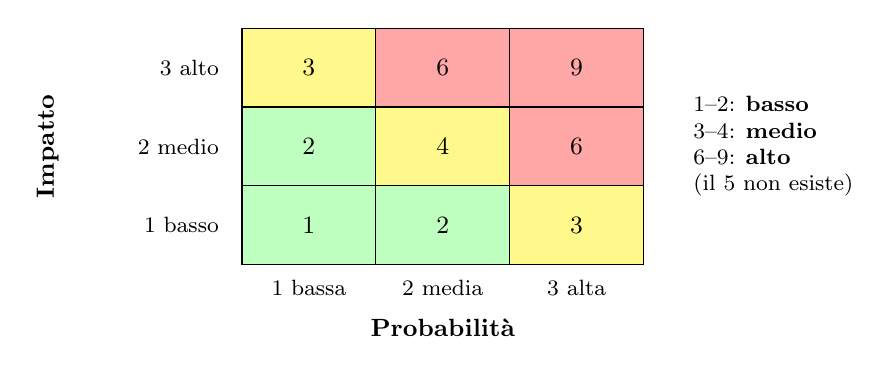
\begin{tikzpicture}[x=1.7cm, y=1.0cm]
  \foreach \pr in {1,2,3}{
    \foreach \im in {1,2,3}{
      \pgfmathtruncatemacro{\scr}{\pr*\im}
      \ifnum\scr<3 \def\cellcol{green!25}\else\ifnum\scr<5 \def\cellcol{yellow!45}\else\def\cellcol{red!35}\fi\fi
      \fill[fill=\cellcol] (\pr-1,\im-1) rectangle (\pr,\im);
      \draw (\pr-1,\im-1) rectangle (\pr,\im);
      \node[font=\small] at (\pr-0.5,\im-0.5) {\scr};
    }
  }
  \node[font=\footnotesize] at (0.5,-0.3) {1 bassa};
  \node[font=\footnotesize] at (1.5,-0.3) {2 media};
  \node[font=\footnotesize] at (2.5,-0.3) {3 alta};
  \node[font=\footnotesize, anchor=east] at (-0.1,0.5) {1 basso};
  \node[font=\footnotesize, anchor=east] at (-0.1,1.5) {2 medio};
  \node[font=\footnotesize, anchor=east] at (-0.1,2.5) {3 alto};
  \node[font=\small\bfseries] at (1.5,-0.8) {Probabilità};
  \node[font=\small\bfseries, rotate=90] at (-1.45,1.5) {Impatto};
  \node[font=\footnotesize, anchor=west, align=left] at (3.3,1.5)
    {1--2: \textbf{basso}\\3--4: \textbf{medio}\\6--9: \textbf{alto}\\(il 5 non esiste)};
\end{tikzpicture}
\end{center}

\paragraph{Livelli di impatto sull'organizzazione (indicazioni del docente).} \textbf{Basso}: perdita
economica limitata, nessun fermo, recupero facile. \textbf{Medio}: un ``mal di testa'' misurabile (sanzioni,
fermo limitato) ma superabile. \textbf{Alto}: evento che può mettere a rischio l'\textbf{esistenza stessa}
dell'organizzazione (perdita totale dei dati senza backup). Le ancore precise della scala 1--3 usate nel
laboratorio sono nel Capitolo~\ref{lab:03}.

\paragraph{Tre dimensioni, un livello.} Con il metodo del corso la probabilità è unica per ogni rischio,
mentre l'impatto si valuta separatamente su \textbf{C}, \textbf{I} e \textbf{A}; si ottengono tre punteggi e
il livello del rischio è il loro \textbf{massimo}:
\[
\text{Livello} = \max\left(P \times I_C,\; P \times I_I,\; P \times I_A\right)
\]

\begin{esame}
\textbf{Errore tipico: fare la media} di C, I, A. Un rischio con punteggi 9/1/1 è \textbf{alto}, non medio:
basta una dimensione alta. E il livello da solo non basta: bisogna sapere \textbf{quale dimensione} lo rende
alto, per scegliere controlli che agiscano su quella (nel Lab~3, R-01 è alto per la riservatezza, R-17 per
la disponibilità).
\end{esame}

\subsection{Rischio inerente e residuo}
\begin{itemize}
  \item \textbf{Rischio inerente}: il rischio come si presenta prima del trattamento in esame. Nel Lab~3 è
    stimato \textbf{con i controlli che l'organizzazione ha oggi} (una baseline debole).
  \item \textbf{Rischio residuo}: il rischio che resta dopo i controlli scelti. Nel Lab~3 si
    \textbf{rivaluta da capo} (nuova probabilità, nuovi impatti), non si calcola ``inerente meno
    efficacia''; probabilità e impatti residui non possono superare gli inerenti.
  \item Anche il residuo è oggetto di decisione: va accettato formalmente, oppure trattato ancora.
\end{itemize}
Lo stesso schema compare nel GDPR: nella DPIA (Capitoli~\ref{lez:2026-09-28} e~\ref{lez:2026-10-05}) il
professore lo riassume come ``residuo = inerente meno mitigazione'', e se il residuo resta alto si passa alla
consultazione preventiva (art.~36) o si ferma il trattamento.

\begin{nota}[Due definizioni di ``inerente'']
Gli appunti 2025/26 definiscono il rischio inerente come quello \emph{in assenza di qualsiasi controllo}; il
materiale del Lab~3 lo stima \emph{con i controlli già in essere}. Sono due convenzioni diffuse: l'importante
è dichiarare quale si usa e applicarla in modo coerente. Gli stessi appunti mettono in guardia dalla
``matrice verde'': mostrare solo il residuo dà l'impressione che tutto sia sotto controllo anche quando il
piano di trattamento non è ancora attuato. Il residuo è ciò che si \emph{spera}, l'inerente ciò che
\emph{c'è}: verificare sempre piano e tempi di attuazione.
\end{nota}

\subsection{Propensione e tolleranza al rischio}
\begin{center}
\small
\begin{tabularx}{\linewidth}{>{\raggedright\arraybackslash}p{2.4cm} X X}
\toprule
 & \textbf{Risk appetite (propensione)} & \textbf{Risk tolerance (tolleranza)}\\
\midrule
Che cos'è & disponibilità complessiva ad assumere rischi per raggiungere gli obiettivi & livello di rischio
  accettato per specifiche attività o processi\\
Livello & strategico: decide il board con l'alta direzione & operativo: soglie e criteri numerici, diversi
  per funzione e tipo di asset\\
Nel Lab~3 & le soglie 1--2 / 3--4 / 6--9 (alto non accettabile) & owner e data obiettivo del singolo
  rischio\\
\bottomrule
\end{tabularx}
\end{center}
Esempio di Gianluca: su una scala 1--9 si accetta ciò che sta sotto 3, il resto va trattato. Nella sua
esperienza, però, quasi nessun rischio inerente che compare in un registro è davvero accettabile così com'è:
i rischi davvero minimi non vengono nemmeno percepiti, e quindi non vengono mappati.

\subsection{Le quattro opzioni di trattamento}
\begin{center}
\small
\begin{tabularx}{\linewidth}{>{\raggedright\arraybackslash}p{2.3cm} X X}
\toprule
\textbf{Opzione} & \textbf{Che cosa significa} & \textbf{Attenzione}\\
\midrule
Mitigare (ridurre) & controlli che riducono probabilità e/o impatto fino a un livello accettabile &
  l'opzione più comune; il residuo va comunque accettato dalla direzione\\
Accettare & nessuna ulteriore misura: il rischio rientra nella propensione o il trattamento costerebbe
  troppo & richiede \textbf{approvazione formale}; un rischio inerente \textbf{alto} non si può accettare\\
Evitare & cessare o non avviare l'attività che genera il rischio & corrisponde allo ``stop del
  trattamento'' visto per la DPIA\\
Trasferire & condividere il rischio con un terzo (assicurazione, outsourcing, SLA) & sposta la perdita
  economica, \textbf{non la responsabilità}; la scelta del terzo va motivata (``non basta una firma su un
  foglio''); la \emph{shared responsibility matrix} del cloud è un trasferimento parziale\\
\bottomrule
\end{tabularx}
\end{center}
Il trattamento è \textbf{strategico}, non solo tattico: non ha senso spendere per mitigare il rischio di un
processo che verrà dismesso a breve. Nella prima lezione Gianluca aveva presentato tre esiti (mitigare,
accettare, trasferire), definendo il trasferimento il ``Santo Graal'' del risk manager; le slide sul risk
management aggiungono \emph{evitare}.

\paragraph{Scegliere i controlli.} Si parte dalla \textbf{minaccia e dagli asset}, mai dal catalogo: quale
controllo interrompe \emph{quella} causa? Si sceglie l'insieme minimo sufficiente, pertinente, efficace e
proporzionato; non si inventa un rischio per dare una ``casa'' a un controllo. La 27002 offre il catalogo e
la guida all'attuazione.

\subsection{Statement of Applicability}
La \textbf{SoA} è un documento \textbf{obbligatorio} per la conformità alla 27001:
\begin{itemize}
  \item elenca \textbf{tutti} i 93 controlli dell'Allegato~A;
  \item per ciascuno dichiara se è applicabile;
  \item ne giustifica l'inclusione o l'esclusione;
  \item ne indica lo stato di attuazione.
\end{itemize}
Documenta le decisioni prese nel trattamento del rischio (quali controlli per quali rischi) ed è centrale
negli audit di certificazione. Per Gianluca conta ancora di più saper giustificare perché un controllo
\textbf{non} è attuato: l'auditor può contestare il legame tra controllo e rischio e chiedere di correggere
la SoA. Il registro va dal rischio al controllo; la SoA dal controllo al rischio.

\subsection{Piano di trattamento}
Per ogni rischio da trattare il piano indica: opzione scelta; azioni concrete; \textbf{owner} di ogni azione;
tempi; risorse (budget e persone: il management chiederà sempre ``quanto costa?''); giustificazione. La
giustificazione discende dalla propensione al rischio:
\begin{itemize}
  \item si \textbf{accetta} perché il rischio è sotto soglia;
  \item si \textbf{mitiga} perché l'inerente è sopra soglia e i controlli portano il residuo entro la soglia;
  \item si \textbf{trasferisce} ciò che resta fuori dal proprio controllo;
  \item si \textbf{evita} quando nessun residuo è accettabile.
\end{itemize}
La matrice RACI è fondamentale nella procedura di gestione dei data breach, ma non è richiesta nel piano di
trattamento.

\subsection{Il risk register}
\label{sec:iso-register}
Il registro dei rischi è un documento \textbf{centrale e vivo} che raccoglie tutti i rischi individuati.
Non ha un formato obbligatorio (Excel o piattaforme dedicate). Campi minimi:

\begin{center}
\small
\begin{tabularx}{\linewidth}{>{\raggedright\arraybackslash}p{4.2cm} X}
\toprule
\textbf{Campo} & \textbf{Perché serve}\\
\midrule
ID univoco & tracciare il rischio in tutti i documenti e progetti\\
Asset coinvolti & sapere che cosa si protegge\\
Minaccia e vulnerabilità & la causa da interrompere: da qui si scelgono i controlli\\
Probabilità e impatto (C, I, A) inerenti & base della valutazione\\
Livello di rischio calcolato & con la matrice; massimo delle tre dimensioni\\
Controlli e misure concrete & azioni, non nomi di controlli (``MFA su tutti i servizi cloud'', non ``8.5'')\\
Giustificazione ed efficacia & perché quelle misure, se agiscono su probabilità o impatto, perché il residuo
  è accettabile\\
Probabilità, impatti e livello residui & dopo il trattamento\\
Decisione di trattamento & una delle quattro opzioni\\
Risk owner & chi decide, firma il trattamento e ne risponde\\
Data obiettivo e ultima revisione & tolleranza del singolo rischio; monitoraggio\\
\bottomrule
\end{tabularx}
\end{center}
\noindent I campi delle slide sono ID, asset, minaccia, vulnerabilità, probabilità, impatto, livello, owner e
trattamento proposto; a lezione Gianluca ha aggiunto la distinzione tra valori inerenti e residui, e il Lab~3
la giustificazione, l'efficacia e le date. Il registro garantisce trasparenza e accountability ed è la base
del trattamento.

\subsection{Monitoraggio continuo e altri framework}
I rischi cambiano, nascono e muoiono: il registro non si chiude in un cassetto. Vanno riesaminati
periodicamente la valutazione, l'efficacia dei controlli, l'avanzamento del piano e i rischi emergenti, in
una vera \textbf{cultura del rischio}. Non serve reinventare la ruota: oltre alla ISO esistono
\textbf{NIST CSF} (funzioni identificare, proteggere, rilevare, rispondere, ripristinare; diffuso negli USA),
\textbf{FAIR} (quantifica il rischio in termini economici), \textbf{OCTAVE} (rischi operativi,
autovalutazione) e le metodologie \textbf{ENISA}, in particolare per i dati personali.

\begin{integrazione}[ISO 31000 e ISO/IEC 27005]
La definizione ``effetto dell'incertezza sugli obiettivi'' viene dalla ISO~31000, la norma generale sulla
gestione del rischio, da cui la 27005 deriva per la sicurezza delle informazioni. La 27005:2022 ammette due
modi di identificare i rischi: \emph{basato sugli asset} (asset, minacce, vulnerabilità: quello del corso) e
\emph{basato sugli eventi} (scenari di alto livello e loro conseguenze, senza partire dall'inventario).
\end{integrazione}

% =====================================================================
\section{Rischio ISO e rischio GDPR/ENISA}
\label{sec:iso-enisa}
% =====================================================================
Il cambio di prospettiva è il punto centrale del risk management del corso. Nel GDPR il rischio si misura
sui \textbf{diritti e le libertà degli interessati}; nella ISO sull'\textbf{organizzazione}. Esempio di
Gianluca: il DPO di un'azienda preoccupato per le conseguenze di un incidente su operatività e processi HR
non ha, solo per questo, un problema di notifica al Garante: sono valutazioni distinte.

\subsection{La metodologia ENISA per i dati personali}
ENISA ha pubblicato, oltre alla metodologia di severità dei breach, linee guida (pensate anche per le PMI)
per valutare il rischio dei trattamenti di dati personali, compatibili con la 27001 e mappate sui controlli
della 27002. Quattro passi:
\begin{enumerate}
  \item \textbf{Contesto del trattamento}: quali dati, finalità, mezzi, luogo (on premise o cloud), categorie
    di interessati, destinatari; tutte le fasi (raccolta, conservazione, uso, trasferimento, cancellazione).
    Risultato: il perimetro della valutazione.
  \item \textbf{Impatto sugli individui}, su quattro livelli: \emph{basso} (piccoli disagi superabili),
    \emph{medio} (disagi significativi: costi, stress, servizi negati), \emph{alto} (conseguenze serie: perdite
    economiche, perdita del lavoro), \emph{molto alto} (conseguenze irreversibili). Si valuta separatamente
    per riservatezza, integrità e disponibilità e \textbf{si prende il più alto}.
  \item \textbf{Probabilità della minaccia} su quattro aree, ciascuna con punteggio 1--3: risorse di rete e
    tecniche; processi e procedure; persone e terze parti; settore e dimensione. Totale 4--5 bassa, 6--8
    media, 9--12 alta.
  \item \textbf{Valutazione del rischio} con la matrice:
\end{enumerate}
\begin{center}
\small
\begin{tabular}{llll}
\toprule
\textbf{Probabilità} & \textbf{Impatto basso} & \textbf{Impatto medio} & \textbf{Impatto alto/molto alto}\\
\midrule
Bassa & basso & medio & alto\\
Media & medio & alto & alto\\
Alta & alto & alto & alto\\
\bottomrule
\end{tabular}
\end{center}
\noindent La matrice ENISA è volutamente prudente: molte combinazioni finiscono in ``alto''. Il livello di
rischio orienta la scelta delle misure ai sensi dell'art.~32.

\subsection{Il confronto}
\begin{center}
\small
\begin{tabularx}{\linewidth}{>{\raggedright\arraybackslash}p{2.5cm} X X}
\toprule
\textbf{Aspetto} & \textbf{ISO/IEC 27001} & \textbf{ENISA (dati personali)}\\
\midrule
Ambito & sicurezza di tutte le informazioni & trattamenti di dati personali\\
Chi subisce l'impatto & l'\textbf{organizzazione} (C, I, A dei suoi asset) & gli
  \textbf{interessati}: diritti e libertà\\
Metodo & libero, purché coerente e documentato & strutturato in quattro passi\\
Probabilità & stimata dall'organizzazione (spesso con threat intelligence) & questionario su quattro aree,
  punteggio 4--12\\
Combinazione di C, I, A & massimo dei tre punteggi (metodo del corso) & massimo dei tre impatti\\
Controlli & 93 controlli dell'Allegato~A, SoA & misure proporzionate al livello di rischio, mappabili sulla
  27002\\
Riferimento & certificazione ISO (volontaria) & art.~32 GDPR (obbligo di legge)\\
Esito tipico & piano di trattamento e registro dei rischi & misure tecniche e organizzative adeguate;
  eventuale DPIA (art.~35)\\
\bottomrule
\end{tabularx}
\end{center}
I due approcci si usano spesso \textbf{insieme}: ENISA per i trattamenti di dati personali, ISO per l'ISMS,
le misure ENISA mappate sui controlli 27002 e un \textbf{unico registro con doppia valutazione}. Il punto di
contatto tra i due piani: un impatto C~=~3 sull'organizzazione, nel Lab~3, è ancorato a un \textbf{breach
da notificare ex art.~33}, cioè a un rischio per gli interessati.

\begin{nota}[Tre strumenti da non confondere]
\begin{itemize}
  \item \textbf{Risk assessment ISO}: rischio per l'organizzazione, \emph{prima} dell'incidente.
  \item \textbf{Valutazione del rischio ENISA per i dati personali} (e DPIA): rischio per gli interessati,
    \emph{prima} del trattamento o dell'incidente.
  \item \textbf{Metodologia ENISA di severità dei breach} (DPC, EI, CB): gravità di una violazione
    \emph{già avvenuta}, per decidere su notifica e comunicazione (Capitolo~\ref{cap:data-breach}).
\end{itemize}
Nel Lab~1 la lezione era la stessa: \textbf{la severità non è il rischio}.
\end{nota}

\begin{integrazione}[Un esempio sui due piani]
Un ransomware cifra il gestionale di uno studio professionale per due giorni, senza esfiltrazione. Lato
ISO: impatto alto sulla \textbf{disponibilità} (scadenze dei clienti mancate, fermo, reputazione), quindi
rischio alto per l'organizzazione. Lato GDPR: è un breach di disponibilità; se i dati si ripristinano dai
backup in tempi brevi e nessun interessato subisce conseguenze, la severità può risultare bassa e non
richiedere notifica, ma la violazione va comunque registrata (art.~33(5)). Stesso evento, due valutazioni,
due registri di riferimento.
\end{integrazione}

% =====================================================================
\section{Errori tipici e messaggi chiave}
\label{sec:iso-errori}
% =====================================================================
\begin{esame}
\textbf{Messaggi chiave del docente}
\begin{itemize}
  \item L'\textbf{ISMS è la base} della 27001: un sistema basato sul rischio e in miglioramento continuo,
    non un timbro. \textbf{I processi contano più dei documenti}.
  \item Numeri: \textbf{93 controlli} in 4 temi (37 / 8 / 14 / 34); clausole \textbf{4--10} non escludibili;
    ciclo di certificazione \textbf{triennale}.
  \item La certificazione riguarda l'\textbf{organizzazione}, è volontaria e non garantisce né sicurezza né
    conformità legale.
  \item Rischio ISO = impatto sull'\textbf{organizzazione}; rischio GDPR/ENISA = impatto sugli
    \textbf{interessati}.
  \item Il risk management è il fondamento della cybersicurezza: asset, minacce, vulnerabilità, impatto,
    probabilità; processo strutturato; trattamento strategico; decisioni documentate nella \textbf{SoA};
    monitoraggio continuo.
  \item Non fermarsi al rischio inerente: la decisione si prende sul \textbf{residuo}.
  \item Ogni scelta (anche l'esclusione di un controllo) va \textbf{motivata e documentata}: conta il
    ragionamento, non il numero.
\end{itemize}
\end{esame}

\begin{esame}
\textbf{Errori tipici}
\begin{enumerate}
  \item Fare la \textbf{media} di C, I, A invece del massimo.
  \item Usare lo stesso impatto per le tre dimensioni senza motivo.
  \item \textbf{Accettare} un rischio inerente alto; lasciare un residuo alto.
  \item Credere che \textbf{trasferire} elimini la responsabilità: si sposta la perdita economica, non
    l'accountability.
  \item Confondere il rischio per l'organizzazione con il rischio per gli interessati (e il risk assessment
    con la severità del breach).
  \item Sottostimare la probabilità di un'organizzazione senza controlli.
  \item Scrivere il nome del controllo al posto della misura concreta; partire dal catalogo invece che dalla
    minaccia.
  \item Residuo uguale all'inerente senza spiegazione, o addirittura superiore.
  \item Pensare che la certificazione 27001 dimostri la conformità a GDPR, NIS2 o CRA.
  \item Escludere controlli scomodi (8.8, 8.12) dalla SoA senza una motivazione solida.
\end{enumerate}
\end{esame}

% =====================================================================
\section{Punti da verificare}
\label{sec:iso-verifica}
% =====================================================================
\begin{verifica}
\begin{itemize}
  \item \textbf{ISO/IEC 27090} (sicurezza dei sistemi di IA): citata a voce come appena approvata; numero e
    stato di pubblicazione da confermare.
  \item \textbf{27017 e 27018}: compaiono nel diagramma della famiglia nelle slide (secondo gli appunti di
    recupero) e negli appunti 2025/26, ma non sono state commentate a lezione quest'anno.
  \item \textbf{PDCA}: secondo gli appunti di recupero il ciclo compare in un'immagine della slide sull'ISMS;
    non è nel testo delle slide né nella trascrizione.
  \item \textbf{Limite dei 21 giorni} e \textbf{sanzione alla Regione} (circa \texteuro{}50.000): dal parlato;
    estremi del documento del Garante e del provvedimento da verificare. Anche la sanzione di
    \texteuro{}500.000 alla banca spagnola per mancata privacy by design.
  \item \textbf{Sovrapposizione 75--80\% con SOC~2} e \textbf{sei mesi} di tempo medio di rilevazione in
    Italia: stime del docente.
  \item \textbf{Linee guida ENISA per le PMI}: titolo e anno del documento non indicati in aula.
  \item \textbf{Tipi di controllo}: a lezione vulnerability assessment e penetration test sono stati
    portati come esempi di controlli \emph{preventivi}; sono anche (e forse soprattutto) attività di
    individuazione delle vulnerabilità. Classificazione da confermare.
\end{itemize}
\end{verifica}
